\section{Les interprétations du phénomène réfraction}
\begin{minipage}[c]{.45\linewidth}
\begin{center}
\end{center}
\input{./lumiereEtMatiere/air-eau.tex}
\end{minipage}
\hfill
\begin{minipage}[c]{.45\linewidth}
\[
n_1 \sin i_1 = n_2 \sin i_2
\]
\end{minipage}

\subsection{Descartes}
\begin{center}
\end{center}
La vitesse suivant x est continue
\[
V_1sin(i_1)=V_2sin(i_2)
\]
\subsection{Fermat}
Le durée du trajet est minimal
\[
\frac{1}{V_1}sin(i_1)=\frac{1}{V_2}sin(i_2)
\]
\subsection{Fresnel}
\begin{minipage}[c]{.45\linewidth}
\begin{center}
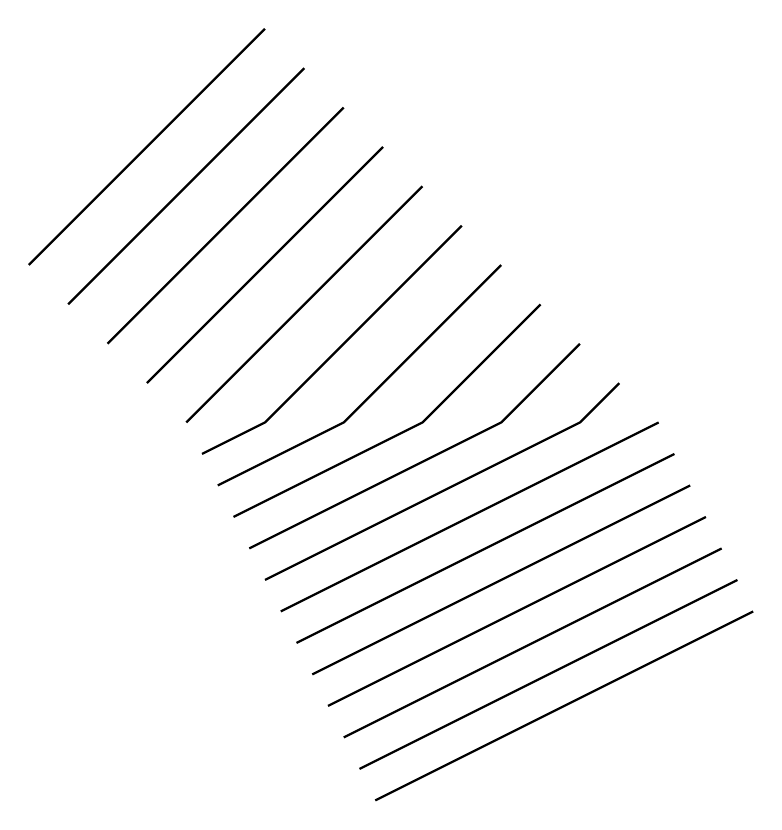
\begin{tikzpicture}

\foreach \k in {0,0.5,...,2}
\draw[thick] (-3-\k, \k) -- (-\k, 3+\k);

\draw[thick] (-2.8, -0.4) -- (-2, 0) -- (0.5, 2.5);
\draw[thick] (-2.6, -0.8) -- (-1, 0) -- (1, 2);
\draw[thick] (-2.4, -1.2) -- (0, 0) -- (1.5, 1.5);
\draw[thick] (-2.2, -1.6) -- (1, 0) -- (2, 1);
\draw[thick] (-2, -2) -- (2, 0) -- (2.5, 0.5);

\foreach \k in {0,0.2,...,1.2}
\draw[thick] (-1.8+\k, -2.4-2*\k) -- (3+\k, -2*\k);

%\draw (1.5, 0.25)[red] node {$\lambda$};
\end{tikzpicture}

\end{center}
\end{minipage}
\hfill
\begin{minipage}[c]{.45\linewidth}
\begin{center}
\end{center}
\end{minipage}

La lumière est une onde, la "longueur d'onde suivant x" est continue. La composante suivant x du vecteur d'onde est continu :
\[
k_1sin(i_1)=k_2sin(i_2) \qquad \frac{1}{\lambda_1}sin(i_1)=\frac{1}{\lambda_2}sin(i_2)
\]
\subsection{De Broglie}
La quantité de mouvement suivant x est continue :
\[
p_1sin(i_1)=p_2sin(i_2) \qquad p=\hbar k \qquad k=\frac{1}{\lambda_1}
\]
